\documentclass[10pt,onecolumn]{MainDocument}

% All KJN's macros and goodies (some shameless borrowing from SPL)
\usepackage{KJN}


%\usepackage[hyphens]{url}

% PDF Info

\ifpdf
\pdfinfo{
	/Title (SOFTWARE ENGINEERING PROJECT: STUDENTS MARKS/RECORDS MANAGEMENT WEBSITE DESIGN)
	/Author (Khosa Masana (559990), Sanele Gcaba(459380), Tshegofatso Misapitso (600313), Londiwe Ngema (448871) )
	/ModDate (D:200510121530)
	/Subject (ELEN417/455 Paper Format, 2005)
	/Keywords (ELEN417, ELEN455, paper, instructions, style guidelines, laboratory project)
}
\fi

%%%%%%%%%%%%%%%%%%%%%%%%%%%%%%%%%%%%%%%%%%%%%%%%%%%%%%%%%%%%%%%%%%%%%%%%%%%%%%%
\begin{document}

	\begin{titlepage}
		
		\newcommand{\HRule}{\rule{\linewidth}{0.5mm}} % Defines a new command for the horizontal lines, change thickness here
		
		\center % Center everything on the page
		{\small School$\;$of$\;$Electrical$\;$and$\;$Information$\;$Engineering,$\;$University of$\;$the$\;$Witwatersrand,$\;$Private$\;$Bag$\;$3,$\;$2050,$\;$Johannesburg,$\;$South$\;$Africa}\\[1.5cm] % Name of your university/college
		
		\textsc{ELEN 4009 - Software Engineering}\\[0.5cm] % Major heading such as course name
		
		\HRule \\[0.4cm]
		{ \large \bfseries Student Marks/Records Management Software}\\[0.4cm] % Title of your document
		\HRule \\[1.5cm]
		
		\large
		
		\textbf{Front end pair :}
		Khosa$\;$Masana$\;$(559990)\ and
		Londiwe$\;$Ngema$\;$(448871)
		
		\textbf{Back end pair :}
		Tshegofatso Misapitso$\;$(600313)\ and
		Sanele$\;$Gcaba$\;$(459380)
		
		
		{\large \today}\\[3cm] % Date, change the \today to a set date if you want to be precise
		
		%\includegraphics{Logo}\\[1cm] % Include a department/university logo - this will require the graphicx package
		
		\begin{figure}[h]
        \begin{center}
        
\includegraphics[scale=0.70]{Wits-logo1}
        \end{center}
        \end{figure}
		
		\vfill % Fill the rest of the page with whitespace
		
	\end{titlepage}
	
	

	\pagestyle{plain}.
	\pagenumbering{roman} 
	\tableofcontents 
	
	\newpage
	
	
	
	%%%%%%%%%%%%%%%%%%%%%%%%%%%%%%%%%%%%%%%%%%%%%%%%%%%%%%%%%%%%%%%%%%%%%%%%%%%%%%%
	%
\section*{Document Status Sheet}
	
	\begin{center}
		\begin{tabular}{ | p{5cm} | p{7cm} |}
			\hline
			\textbf{Document Title}& Software Requirements, Front and Back end development documentation \\ \hline
			\textbf{Authors} & M.$\;$Khosa, S.$\;$Gcaba, T.$\;$Misapitso, L.$\;$Ngema \\ \hline
			\textbf{Version} & 1 \\ \hline
			\textbf{Document Status} & Final  \\ \hline
			
		\end{tabular}
	\end{center}
	
	
	\begin{center}
		\begin{tabular}{ | p{2cm} | p{3cm} | p{5cm} | p{5cm} |}
			\hline
			\textbf{Version}& \textbf{Date}& \textbf{Author(s)} & \textbf{Summary} \\ \hline
			0.0.1 & 25-02-2016 & M.$\;$Khosa, S.$\;$Gcaba, T.$\;$Misapitso, L.$\;$Ngema& Document Creation. \\ \hline
		    1 & 11-04-2016 & M.$\;$Khosa, S.$\;$Gcaba, T.$\;$Misapitso, L.$\;$Ngema& Final Documentation with edited requirements as per project owner's request. \\ \hline
		\end{tabular}
	\end{center}
	
	\newpage
	
	
	%%%%%%%%%%%%%%%%%%%%%%%%%%%%%%%%%%%%%%%%%%%%%%%%%%%%%%%%%%%%%%%%%%%%%%%%%%%%%%%
	%
	\pagestyle{plain}.
	\pagenumbering{arabic} 

%%%%%%%%%%%%%%%%%%%%%%%%%%%%%%%%%%%%%%%%%%%%%%%%%%%%%%%%%%%%%%%%%%%%%%%%%%%%%%%
%
\section{INTRODUCTION}

\subsection{Problem Statement}

University of the Witwatersrand school of electrical engineering and Information Engineering aims on implementing a software to manage  provisional students marks as they complete assignments, tests, laboratory work, etc., throughout the year. The software to be implemented will have three distinct users which are the course coordinator, the school administrator and the student. Each user has different levels of access to the database. The course coordinator of each course, offered  by the school, must be able to enter marks obtained by students for all forms of assessment like tests, assignments, labs, exams and many more depending on the structure of a particular course. Students must be able to retrieve and view their assessment marks obtained so far, for all forms of assessment on each course. This allows students to track  their progress throughout the year as they continuously check their marks on the system. The school administrator must be able to retrieve relevant summaries of marks for each course in a spread-sheet format which will be analysed by the course coordinator and the head of school and then be sent to the official mark system of the faculty. All the marks stored, for each course, in an academic year must be kept in the database for 10 years. The users must be able to interact with the database through a web browser and a smart mobile application. 
 
\subsection{Project Objectives}

The objective of this project is to design, implement and develop a student marks software that is user-friendly and cost effective. The software has only three types of users which are the course coordinator, school administrator and a student. The users must interact with the database through a web browser. The software must be able to allow the course coordinator, of each course offered by the school, to input marks obtained by the students for all forms of assessments. The students must be able to access the software and retrieve their marks throughout the year. The school administrator must be able to retrieve relevant summaries of marks for each course in a spreadsheet format. The project will be divided into two parts namely the back-end and front-end. The front-end of the software is going to be developed using HTML, CSS, JavaScript and PHP. The back-end is developed using PHP and mySQL. The two parts are thereafter combined into one student record/mark system. There is no budget allocated to this project since it can be designed, implemented and developed using readily available resources such as computers. The server used is an open source Apache server. The time allocated to complete this project is 2 months and 3 days, From 9th of February to the 11th of April. 

\subsection{Stakeholders}

Figure 1 shows the stakeholders for the project. 


\begin{figure}[h]
\begin{center}
\includegraphics[scale=0.70]{stakeholders}
\caption{Project Stakeholders}
\end{center}
\end{figure}

\subsection{Deliverables}

\textbf{At the end of this project the application website is expected to atleast enable users to:-}
\begin{itemize}
\item Register themselves.
\item Identify which group among the three mentioned above the user belongs to.
\item If the user is a student, the most important thing is for them to track their progress by having all their marks on the system.
\item It is important for the Admin to retrieve a table of student names and their results.
\item Another important task for the Course Co-ordinator is for him/her to add various forms of assessment and also input the student marks.
\end{itemize} 


\clearpage
\newpage
\section{Requirements Gathering}

\subsection{Methodology}

The System Development Life Cycle (SDLC) methodology to be used for the project follows the Agile Model, this model breaks down the product into a cycle, it quickly delivers a working product and is a more realistic methodology. Ongoing releases are produced with small incremental changes and it depends heavily on customer interaction \cite{ref7}. Specifically the Scrum Agile Model will be adopted for the project, Scrum comprises of short sprints and it enables the software team to be able to prioritize on what matters most. The Scrum Model is basically about delivering more often and responding to feedback regularly offered\cite{ref8}.           

\subsection{Purpose}

The purpose of this document is thus to present a detailed description of the requirements, design and implementation of the student marks/record system (SMMS). It will state the purpose and features of the system, the interfaces of the system, what the system will do, the limitations under which it must operate, define inputs and the expected reaction of the system (that is the outputs of the system) and present the designed and implemented web application back-end and front-end subsystems. 

Student Marks/Records Management Software provides on-line services that enable students to view their marks as they complete  assignments, tests and laboratory work, the software system allows staff such as course coordinators the right to add/edit marks obtained by the student under different forms of assessment. It is a convenient way for students to have access to their marks in a safe and confidential way as opposed to accessing them on notice boards where everyone else can publicly see them. The system ensures that each student can track his/her tentative progress throughout the year,it also helps in establishing errors in the record as early as possibly. 

\subsection{Project Scope}
\begin{itemize}

\item There are three basic users of the system - Students, Course coordinators and School administrator.
\item The primary function of the application is to allow students and staff  to log-in using their details (Student/Staff number and password) and be able to access and view student records, the records include student marks for all forms of assessments for all courses registered for. 
\item The system database stores user profiles and student marks records. Marks records are retained for a period of 10 yrs.
\item The software program should have domains assigned, i.e. each user can be able to access relevant information and they are allowed to view/edit/add based on what their recognised domain.
\item  The system would be accessed online via a Browser.

\end{itemize}

Below is a list of privileges per user as specified on the project brief \cite{ref9}.

\textbf{The Course Coordinator should be able to:-}
\begin{itemize}
\item Register himself/herself.
\item Add various assessment method for the course and weighting for each assessment.
\item Enter student marks on a user-friendly interface.
\item Display or print out the table of students and their marks.
\item Generate a summary statistics of the performance of the students - maximum, minimum, average, standard deviation or variants of each assessment.  
\item View projected pass rate based on the assessment marks accumulated students in class.
\end{itemize}

\textbf{The School Administrator should be able to:-}
\begin{itemize}
\item Register himself/herself.
\item Display or print out table of students and their marks.
\item Generate a summary statistics of the performance of the students. 
\item Generate a comparative chart of the assessment marks of selected courses being taken by students of a particular group. 
\item Histogram of assessment marks of all courses taken by a specific student.   
\item Any recorded offences (e.g. plagiarism) for a student.
\item The performances in the same course across different years may be compared.
\end{itemize}

\textbf{The Student should be able to:-}
\begin{itemize}
\item Register himself/herself.
\item Display assessment marks for a course and statistics for that assessment.
\item Display assessment marks for all the courses  
\item Based on current assessment marks, give what performance goals are needed to pass the course.
\end{itemize}

\subsection{List of Definitions and abbreviations}

\subsubsection{Definitions}
\begin{center}
    \begin{tabular}{ | p{3cm} | p{9cm} |}
\hline
\textbf{Term}& \textbf{Definition}\\ \hline
 Database & A collection of records stored within the system \\ \hline
 Table & A collection of related data consisting of columns and rows \\ \hline   
 Client & A requesting program or a user\\ \hline 
     \end{tabular}
\end{center}

\subsubsection{Abbreviations}~\\

\textbf{SMMS} - Student Marks/record management system

\textbf{HTTP} - Hypertext Transfer Protocol

\textbf{HTML} - HyperText Markup Language

\textbf{RDBMS} - Relational Database Management System

\textbf{SQL} - Structured Query Language

%%%%%%%%%%%%%%%%%%%%%%%%%%%%%%%%%%%%%%%%%%%%%%%%%%%%%%%%%%%%%%%%%%%%%%%%%%%%%%%
%
\subsection{Tools used}
\textbf{Web server} - Apache2

The Apache web server is the worlds most used web server software program, it uses HTTP to serve files that form web pages to users in response to their requests. It is an open source program \cite{ref5, ref6}. 

\textbf{Development tools (Front-End)} - HTML, CSS and Javascript

\textbf{Development tools (Back-End)} - PHP  

PHP is a server scripting language, it is widely used, free, and efficient tool.

\textbf{Database Platform} - MySQL and PHPmyadmin 

MySQL is an open-source RDBMS, it stores data in tables and PHPmyadmin is a graphical tool intended to handle administration of MySQL over the web, while phpMyadmin provides a user interface for the mySQL RDBMS.  

\subsection{Expanded Description of the project}

The software system will follow a Two-Tier Architecture due to its ease of use and maintainability as compared to a Three-Tier Architecture. However, the performance of a Two-Tier Architecture slows down with an increase in users \cite{ref3}, hence a Three-Tier Architecture will be implemented with an increase of the number of users. Figure 2 below shows the Two-Tier Architecture for the student marks/record system.   
\begin{center}
\begin{figure}[h]
\centering
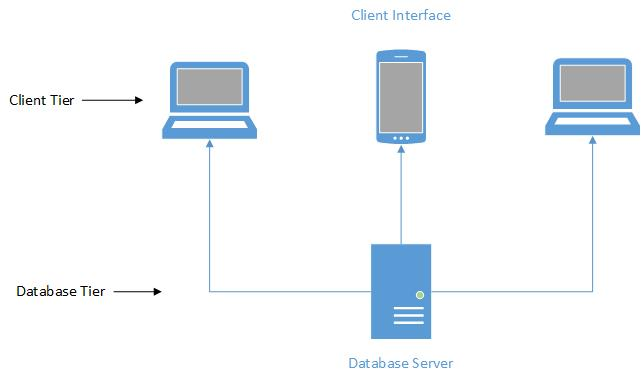
\includegraphics[width=10cm]{Two-Tier}
\caption{Two-Tier Software Architecture}
\end{figure}
\end{center}

A Two-Tier Architecture is a software architecture where the interface runs on a client and the data layer is stored on a server\cite{ref4}.



\subsection{Constraints }
\begin{itemize}
\item The User Interface language is English only.
\item The program currently runs on a localhost.
\end{itemize}

\subsection{ER Diagrams }
The ER Diagrams below show how data is organized within the database.

\begin{center}
\begin{figure}[h]
\centering
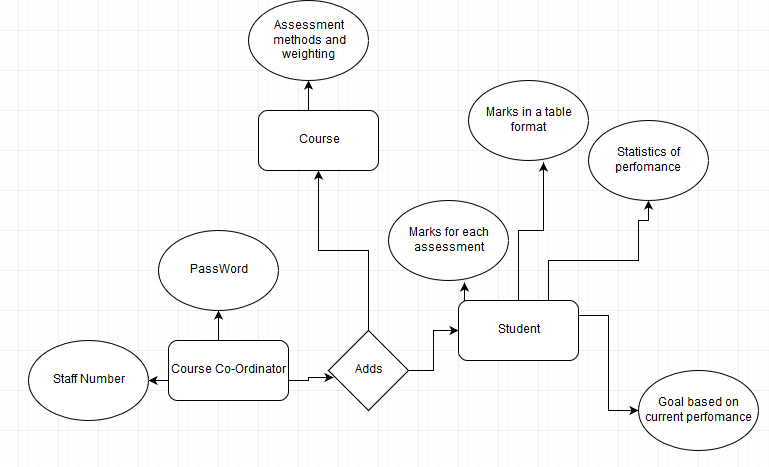
\includegraphics[width=10cm]{ER1}
\caption{ER Diagram for Course co-ordinator and student}
\end{figure}
\end{center}

\begin{center}
\begin{figure}[h]
\centering
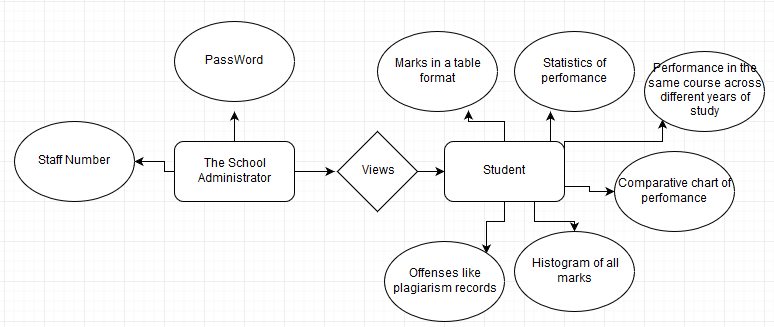
\includegraphics[width=10cm]{ER2}
\caption{ER Diagram for the administrator and student}
\end{figure}
\end{center}

\newpage

\begin{center}
\begin{figure}[h]
\centering
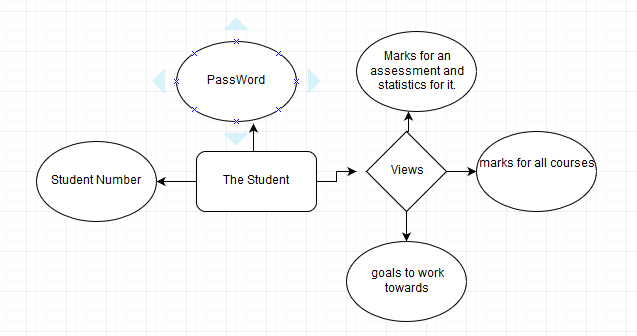
\includegraphics[width=10cm]{ER3}
\caption{ER Diagram for student}
\end{figure}
\end{center}

\subsection{Hardware Specifications }
\textbf{Minimum Requirements}
\begin{center}
	\textbf{Client side}\\
	\begin{tabular}{ | p{5cm} | p{4cm} | p{3cm} | p{3cm} |}
		\hline
		\textbf{Windows} & \textbf{Processor} & \textbf{RAM} & \textbf{Disk Space}\\ \hline
		Internet Explorer	&	Intel Pentium III	
		or AMD - 800 MHz	&	128 MB	&	100 MB		\\ \hline
		Google Chrome		&	Intel Pentium IV - 
		SSE2 capable		&	128 MB	&	100 MB		\\ \hline
	\end{tabular}
	
	
	\begin{tabular}{ | p{5cm} | p{4cm} | p{3cm} | p{3cm} |}
		\hline
		\textbf{Mac} & \textbf{Processor} & \textbf{RAM} & \textbf{Disk Space}\\			\hline
		Google Chrome		&	64 bit Intel  
		processor	       &   128 MB  &	100 MB	\\ \hline
	\end{tabular}
	
	
	\begin{tabular}{ | p{5cm} | p{4cm} | p{3cm} | p{3cm} |}
		\hline			\textbf{Linux} & \textbf{Processor} & \textbf{RAM} & \textbf{Disk Space}\\
		\hline
		Google Chrome		&	Intel Pentium III  
		processor	       &   128 MB  &	100 MB	\\ \hline
	\end{tabular}
	
	\textbf{Server side}\\
	\begin{tabular}{ | p{5cm} | p{4cm} | p{3cm} | p{3cm} |}
		\hline	
		\textbf{Linux} & \textbf{Processor} & \textbf{RAM} & \textbf{Disk Space}\\
		\hline
		Apache 2		&	2 GHz processor or faster  
		processor	       &   1 GB (32 bit) or 2 GB (64 bit)  &		\\ \hline
	\end{tabular}
\end{center}

\textbf{Recommended Requirements}
\begin{center}
	\textbf{Client side}\\
	\begin{tabular}{ | p{5cm} | p{4cm} | p{3cm} | p{3cm} |}
		\hline
		\textbf{Windows} & \textbf{Processor} & \textbf{RAM} & \textbf{Disk Space}\\ \hline
		Internet Explorer	&	1 GHz or faster	&	1 GB (32 bit) or 2 GB (64 bit)	&	256 MB		\\ \hline
	\end{tabular}
	
	
	\begin{tabular}{ | p{5cm} | p{4cm} | p{3cm} | p{3cm} |}
		\hline
		\textbf{Mac} & \textbf{Processor} & \textbf{RAM} & \textbf{Disk Space}\\				\hline
		Google Chrome	&	64 bit Intel processor	 &  1 GB  &	256 MB	\\ \hline
	\end{tabular}
	
	
	\begin{tabular}{ | p{5cm} | p{4cm} | p{3cm} | p{3cm} |}
		\hline
		\textbf{Linux} & \textbf{Processor} & \textbf{RAM} & \textbf{Disk Space}\\
		\hline
		Google Chrome		1 GHz or faster	&	1 GB (32 bit) or 2 GB (64 bit)	&	256 MB	\\ \hline
	\end{tabular}
	
	
	\textbf{Server side}
	Server specifications will depend on the development of the project.
\end{center}


%Student record/marks system
%Backend Documentation by Masana Khosa (559990) and Londiwe Ngema (448871)

\section{Part A : Front-end}

This section presents the design of the user interface of the software. The user interface provides a visual platform for all the users. It provides a more user friendly environment to the client's database queries. The users are able to read and write from and into the database through the user interface. The user interface was implemented using HTML, JavaScript, CSS, and PHP. HTML was used for designing attributes or objects on user interface platforms. JavaScript was used for the animations on the welcome page. CSS gives application its custom look. PHP was used to help users query the database through the user interface. 

The user interface consist of a login page. In the login page, all the users will be asked to input login details and that includes the user-name, password and domain. The login details will be queried into the database to see if they are valid. If the login details are not valid, an error message will be displayed to the user. If the login in details are valid, the user will be redirected to a specific page according to the specified domain. If the user is a course coordinator, the user will be redirected to a course coordinator page, if the user is an administrator, the user will be to an administrator page and same applies for the student. The page where a user will be redirected to depends on the domain specified. Each page where users will be redirected to has a logout button that takes the user back to the login home page. 


\subsection{Login page design}

HTML: Different HTML tags used to describe HTML documents were used to describe the login page. The login page consists of the welcome text and wits pictures to create a more attractive but simple welcome page. A form with input tags for users to input the user-name and password was placed on the login page. The form also consist of a drop-down tag to select the domain. A submit button was also placed to submit the form with login details.

CSS: A CSS file was made for the home page. All the tags mentioned above were given an "id" which is used for reference in the CSS file. In the CSS file for the login page, each tag was given a position, colour, opacity, background colour and all the other styling necessary. 

JavaScript: When the login page is opened, a welcome title slides in from the left of the page up until the middle of the page, when the welcome tittle is done sliding, a wits logo is displayed behind the welcome statement. All theses animations of objects on the login page were done using JavaScript.    

     
PHP: PHP receives the posted form that has the login details of a specific user after when the user presses the submit button. The login details in the form are then sent to the database for verification. If the login details are valid, the user is then redirected to either a student page, course co-ordinator page or administrator page depending on the domain specified.   

\subsection{Student page design}

HTML: The student page was designed to be more user friendly. The student page consists of a menu section where the student can select the options based on their level of access. All the options in the menu section are hypertext references that redirect the student to a specific page based on the selected option. Adjacent to the menu section is a 'more-information' section that explains in detail what each of the menu options is for.

The options in the menu section are:-

\begin{itemize}
\item Assessment marks for a course
\item Statistics
\item Assessment  marks for all courses
\item Performance goals
\end{itemize} 


CSS: The styling of each attribute on the student page was defined on the CSS file.

PHP: When each of the hypertext references in the menu section is clicked, the student is redirected to a specific page depending on the option chosen. When a student selects assessment marks for all courses option, his/her student number will be used to query a table with final marks associated with that student number and the final marks for each course will be displayed to the student. When the student selects the statistics option, the student will be redirected to a page where pass rates and other statistics of each course will be displayed. When a student selects the assessment marks for a course option, the student will be redirected to a page where a list of courses which that particular student is doing will be displayed. When a student selects a particular course, marks for all forms of assessments (labs, assignments, tests and exams) for the course selected will be displayed. And lastly, when the student selects the performance goals option, the student will be redirected to a page that displays a message on how to improve based on their current marks.

\subsection{Course Coordinator page design}

  
HTML: The course coordinator page consist of a menu section with options limited to his/her privileges. Adjacent to the menu section is a 'more-information' section that further explains the options that can be selected by the course coordinator. 

The options that are in the menu section are

\begin{itemize}
\item Assessment Methods
\item Student Marks
\item Table of Students 
\item Statistics
\item Pass rate
\end{itemize}

CSS: All the styling for the attributes in the course coordinator page were defined in the CSS file.

PHP: PHP was used to redirect the course coordinator to appropriate pages when a selection on the menu is made. When the course coordinator selects the Assessment methods, the coordinator will be redirected to a page where he/she will be allowed to upload documents with the assessment methods and the weighting for each assessment. When the course coordinator selects the student marks option, the course coordinator will be redirected to a page where he will be allowed to print the a table of students and their marks.
When the course coordinator selects the table of the students option, he/she will be redirected to a page to enter the marks of students into the database. The statistics option will redirect the course coordinator to a page where there is a summary of statistics for each course to be displayed. Lastly, the pass rate option will redirect the course coordinator to a page where the pass rate of the course will be displayed. 
%%%%%%%%%%%%%%%%%%%%%%%%%%%%%%%%%%%%%%%%%%%%%%%%%%%%%%%%%%%%%%%%%%%%%%%%%%%%%%%
%
\subsection{Head of School/Administrator page design}

HTML: The administrator page consists of a menu section with options of things that an  administrator can do. Adjacent to the menu section is the 'more-information' section where each option is further explained. 

The menu section on the administrator page has the following options. 

\begin{itemize}
\item Table of students
\item Statistics
\item Comparative chart
\item Histogram
\item Offences
\item Performance comparison
\end{itemize}

CSS: A CSS file was created for the administrator page. All the styling of the attributes in the administrator page were designed in the CSS file. 

PHP: The option: table of students, statistics and table of students work the same way as described in section 2.3 (Course Coordinator page design). The histogram option redirects the administrator to a page where a histogram of assessment marks of all courses taken by a specific student will be displayed. The Offences options will redirect the administrator to a page where a downloadable pdf file with all offences,like plagiarism, committed by students will be recorded. The performance comparison option redirects the administrator to a page where the administrator will be asked specify a course, after the course name has been specified, a graph showing pass rate percentages for the past ten year for the specified course will be displayed.      


\subsection{Use case diagrams}



\subsubsection{Student Use-Case Report}$\;\;\;\;\;\;\;\;\;\;\;\;\;\;\;\;\;\;\;\;\;\;\;$
	
	A use case report for a student is shown in Figure 2.
	\begin{center}
		\begin{figure}[h]
			\centering
			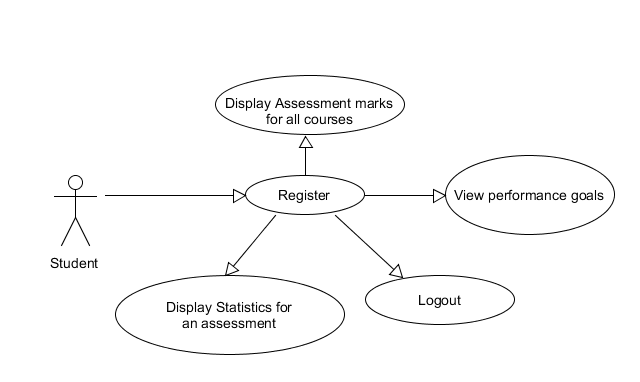
\includegraphics[trim={0cm 0cm 0cm 0cm },clip,scale = 1.1]{StudentUsecase}
			\caption{Use Case Diagram For Student}
		\end{figure}
	\end{center}
	
	
	
	\begin{center}
		\begin{tabular}{ | p{3cm} | p{10cm}| }
			\hline
			\textbf{Use case}& \textbf{Description} \\ \hline
			Register & The student need to sign in in order to view the results \\ \hline
			Display assessment marks & A student must be to display assessment marks for all courses  \\ \hline
			Statistics for an assessment & A student must be able to display assessment marks for a course and the statistics for that assessment \\ \hline
			View performance goals & A student must be able to view what perfomance goals are needed to pass pass the course based on current assessment \\ \hline
			Logout          & The student must be able to logout  \\ \hline
			
		\end{tabular}
	\end{center}
	\clearpage
	\subsubsection{Course Coordinator Use-Case Report}$\;\;\;\;\;\;\;\;\;\;\;\;\;\;\;\;\;\;\;\;\;\;\;$
	
	A use case report for Course Coordinator is shown in Figure 3.
	\begin{center}
		\begin{figure}[h]
			\centering
			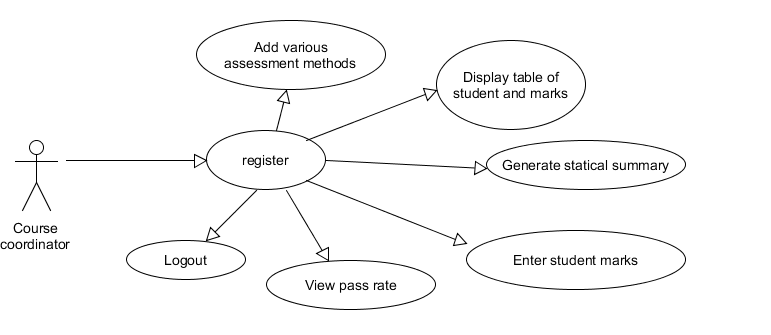
\includegraphics[trim={0cm 0cm 0cm 0cm },clip,scale = 0.85]{CourseCoordinatorUsecase}
			\caption{Use Case Diagram For Staff}
		\end{figure}
	\end{center}
	
	
	
	\begin{center}
		\begin{tabular}{ | p{3cm} | p{10cm}| }
			\hline
			\textbf{Use case}& \textbf{Description} \\ \hline
			Register & Staff need to sign in order to modify results \\ \hline
			Add various assessment methods & Add various assessment method for the course and the weighting for each assessment  \\ \hline
			
			Display table of student and marks & Display or print out the table
of studets and their marks\\ \hline
            Generate statical summary & Generate A summary statistics of the perfomance of each student  \\ \hline
            Enter student marks & Enters the student's marks for each assessment in a user-friendly interface \\ \hline
            View pass rate & View projected pass rate based on the assessment marks accumulated by the students in the class thus far \\ \hline
			Logout          & Coordinator member must be able to logout  \\ \hline
			
		\end{tabular}
	\end{center}
	
	
	
	
	\clearpage
	\subsubsection{Administrator Use-Case Report}$\;\;\;\;\;\;\;\;\;\;\;\;\;\;\;\;\;\;\;\;\;\;\;$
	
	A use case report for an Administrator is shown in Figure 4.
	\begin{center}
		\begin{figure}[h]
			\centering
			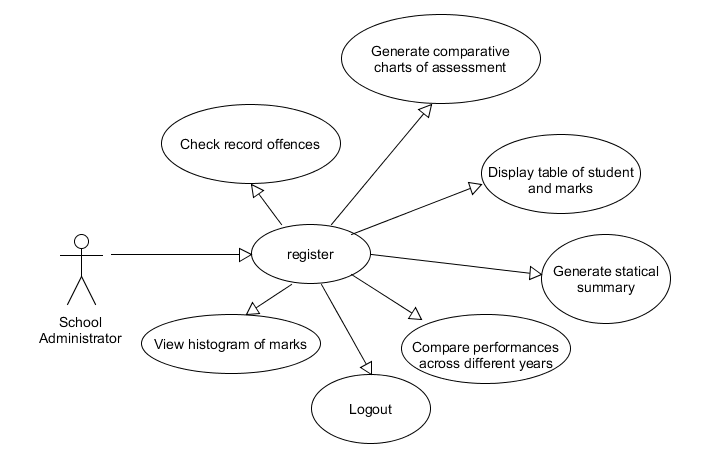
\includegraphics[trim={0cm 0cm 0cm 0cm },clip,scale = 0.85]{AdminUsecase}
			\caption{Use Case Diagram For Administrator}
		\end{figure}
	\end{center}
	
	
	
	\begin{center}
		\begin{tabular}{ | p{3cm} | p{10cm}| }
			\hline
			\textbf{Use case}& \textbf{Description} \\ \hline
			Register & Administrator need to sign in \\ \hline
			Check record offences & The administrator must be able to check any record offences like plagiarism for a student   \\ \hline
			Generate comparative charts of assessment & Generate a comparative chart of the assessment marks of selected courses 
being taken by students of a particular group \\ \hline
Display table of student and marks & Display or print out the table
of studets and their marks\\ \hline
Generate statical summary & Generate A summary statistics of the perfomance of each student  \\ \hline
Compare performances across different years & compare performances in the same course across different years \\ \hline 
View histogram of marks & View a histogram of assessment marks
of all courses taken by a specific specific student  \\ \hline 

			Logout          & Administrator must be able to logout  \\ \hline
			
		\end{tabular}
	\end{center}
	
	\newpage
	\section{Sequence Diagram}
	
	The sequence diagram in Figure 5 shows Sequence diagram of a student.  
	
	
	\begin{center}
		\begin{figure}[h]
			\centering
			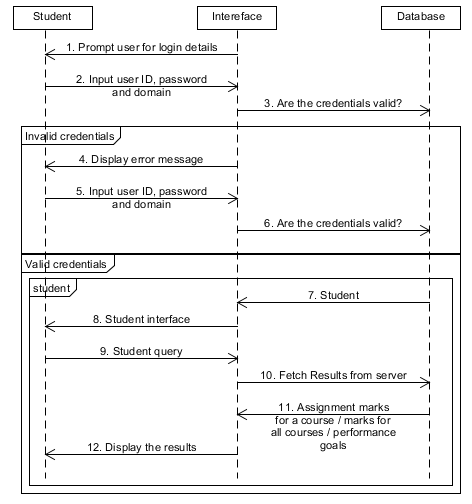
\includegraphics[trim={0cm 0cm 0cm 0cm },clip,scale = 1.3]{StudentSequence}
			\caption{Student Sequence Diagram}
		\end{figure}
	\end{center}
	\newpage
	
	
	The sequence diagram in Figure 6 shows Sequence diagram of an administrator.  
	
	
	\begin{center}
		\begin{figure}[h]
			\centering
			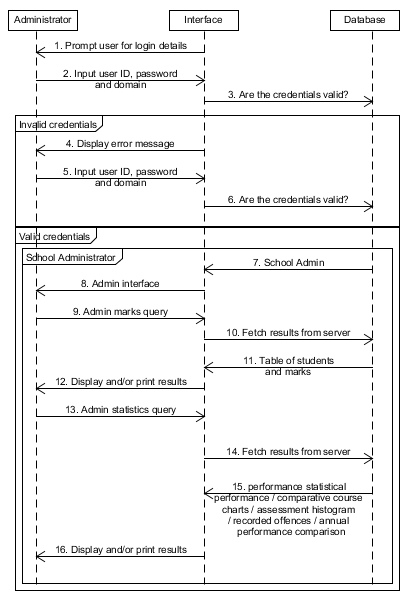
\includegraphics[trim={0cm 0cm 0cm 0cm },clip,scale = 1.1]{AdministratorSequence}
			\caption{ Administrator Sequence Diagram}
		\end{figure}
	\end{center}
	\newpage
	
		The sequence diagram in Figure 7 shows Sequence diagram of an course coordinator.  
	
	
	\begin{center}
		\begin{figure}[h]
			\centering
			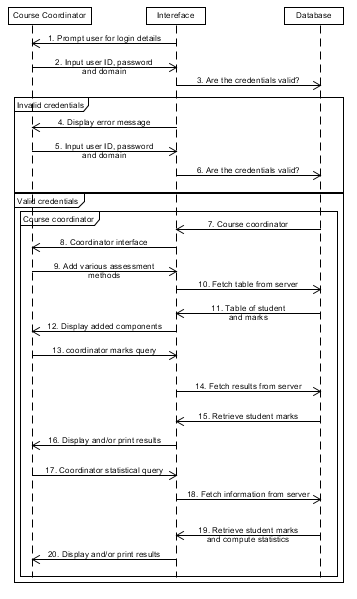
\includegraphics[trim={0cm 0cm 0cm 0cm },clip,scale = 1.1]{CoordinatorSequence}
			\caption{Course Coordinator Sequence Diagram}
		\end{figure}
	\end{center}

 % Front-End Documentation by Masana Khosa And Londiwe Ngem

\newpage

%Student record/marks system
%Backend Documentation by Sanele Gcaba (459380) and Tshegofatso Misapitso (600313)


\section{Part B : Back-End}  
The Back-End constitute of three parts, these include the server,the database, and the application(Generally referred to as the business model), hence the  student marks/record system is designed following a two tier architecture as described in the requirements gathering section. The developed Back-End follows a LAMP web development architectural design. That is, \textbf{L}inux is used as the operating system for the server to run on, \textbf{A}pache is deployed as the application server, \textbf{M}ySQL is used as the Relational SQL Database Management System (RDBMS) and \textbf{P}HP is used as a scripting server Language for realising the designed business model or application requirements as per user specification.     

\subsection{The Server}
The Apache server is used to serve the web-pages that are designed and implemented by the front-end development team, this server is hosted within a Personal Computer (PC) and accessible using a local host of the machine. For the presented web application system, the Apache server is run on a Linux operating system. The Linux operating system is specifically chosen for the server to run on because of its Stability, Security and low Cost of operation \cite{ref1}. As a result a PC running Linux Ubuntu operating system was chosen to host the server. The used Apache server is chosen because it is easy to install and operate, it also provides a secure, efficient HTTP services. Moreover, Apache is a thoroughly tested server partly because of its wide use, serving over a half of all the websites in the World Wide Web (WWW). The Server is open source and it provides free HTTP services.  

\subsection{The Database} 

The project requires that data is stored and later on read from or edited depending on the logged on user, to achieve this, there are multiple datasets that need to be considered and implemented. 
The RDBMS was chosen for implementation due to its advantages over typical Flat file database systems, flat file database systems are limited by the number of tables the database can hold, only one table per flat file can be implemented, it is thus prone to data duplication and data corruption \cite{ref10, ref11}. 

However RDBMS allow the implementation of multiple tables that are related, this ensures that storage of large amount of data is possible. RDBMS enables organising the large amount of data and defining the relationship between the tables based on the defined business model. MySQL RDBMS was thus chosen because it is an open source database that is well documented and widely used\cite{ref2}. PHPMyadmin was used in order to provide an easy to use interface for the database design. Two databases were designed and implemented for the student mark/record system. In order to design these databases, it is important to analyse the data to be stored and how the data will be used.

\subsubsection{Database Design}~\\

The multiple data sets to be stored in the databases are as a result of:
\begin{itemize}
\item Users that include the course coordinator, student and school administrator who need to be able to register themselves. This implies that the database should store login details for all the users, additionally there should be information to distinguish between these users. Due to this business model or requirement, a database for users was created, it was created as a separate database considering possible future login requirements for future applications.

As shown in the figure below, the database has a user table that has the Username, Password and Domain as columns. The three columns in this table are necessary to identify the user logging in. The domain column is essential in defining the role of a user logged in, hence based on this column, a relevant page is redirected to.
\clearpage
\begin{center}
\begin{figure}[h]
\centering
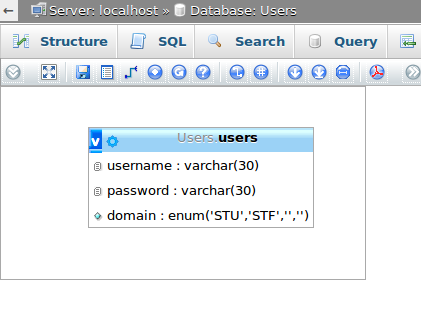
\includegraphics[width=10cm]{Users}
\caption{Users database and table }
\end{figure}
\end{center}

The possible improvement in this user database design would be storing the password as an encrypted password rather than storing it as is, this would be done to improve system security considering the confidentiality of the information stored within the students record/marks system.  
 
\item The student information, individual course information, course components and their percentage contribution form part of a student record database system. 

\begin{center}
\begin{figure}[h]
\centering
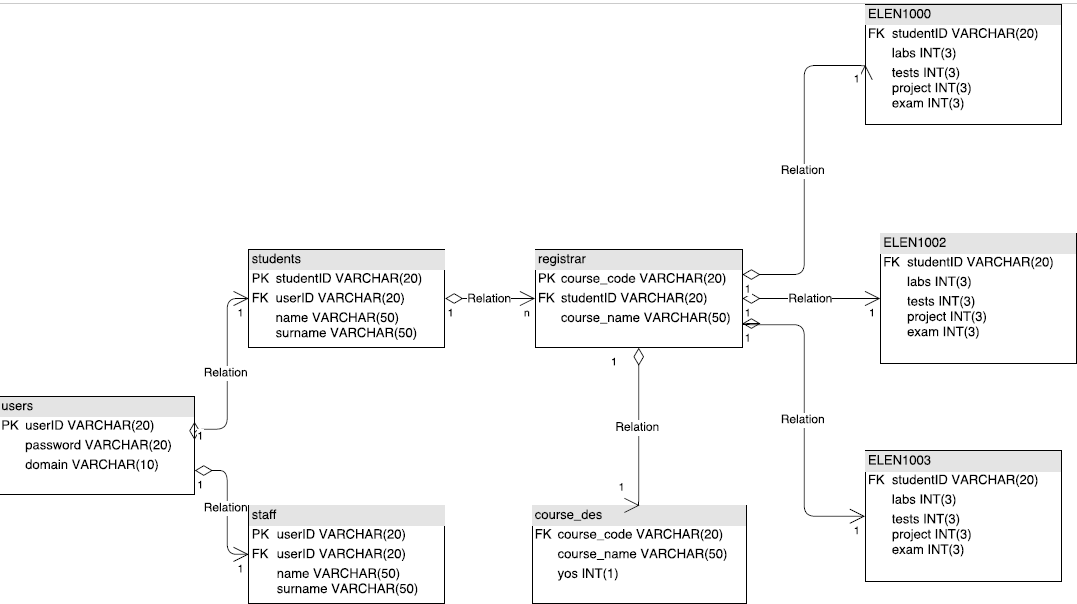
\includegraphics[width=14cm]{OverallDesign}
\caption{Student record Database design}
\end{figure}
\end{center}

\clearpage
\textbf{Students :}

This table is meant to store each individual student's information that include the student's name, surname and studentID which is a unique key that can be used to identify a student. This table has an auto incremented id as a primary key.  

\begin{center}
\begin{figure}[h]
\centering
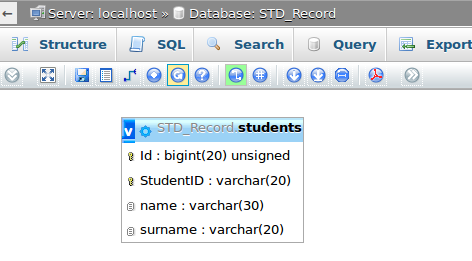
\includegraphics[width=10cm]{Students}
\caption{Students}
\end{figure}
\end{center}


\textbf{course$\_$description :}
This table contains the course code and course name, as the name suggests, it provides a description of each individual course in details. The course code is related to the course name in this table, each course code is unique and thus defined as such in the database.  

\textbf{registrar : }
This table is a logic table which is populated based on student registration business logic. This is specifically for student registration to a particular course, it constitute of a studentID and course$\_$code. On registration, the studentID is paired to a specific course$\_$code registered and the table's primary key is the id which is an auto incremented value.

\begin{center}
\begin{figure}[h]
\centering
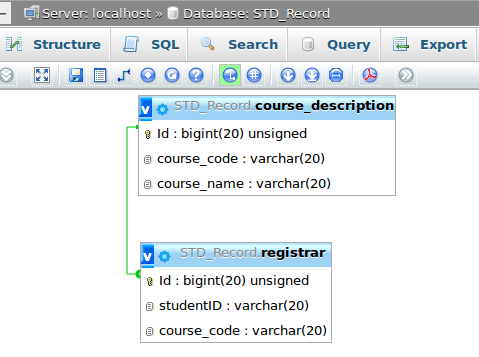
\includegraphics[width=8cm]{descriptionAndRegistar}
\caption{Course description and Registration}
\end{figure}
\end{center}

\clearpage
\textbf{staff : }
The staff table has a userID, this a unique variable, a staff name and surname as well as courses the lecture coordinates. An assumption that each individual lecture can not coordinate more than four courses was made to simplify the application due to implementation time constraint. However, an improvement in future versions would not make that assumption, instead lectures will be able to coordinate a non constant defined number of courses unless the business logic specifically require this to be the case.        

\begin{center}
\begin{figure}[h]
\centering
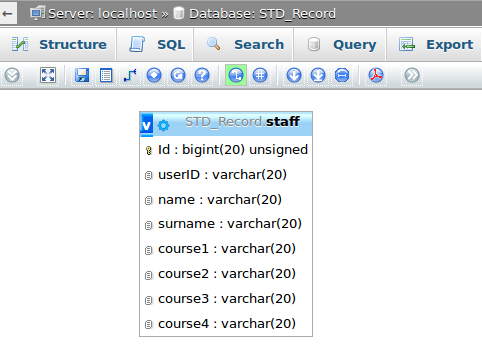
\includegraphics[width=8cm]{Staff}
\caption{Staff table}
\end{figure}
\end{center}

\textbf{courses : }
In order to simplify the problem due to time constraints, each course is designed to have its own individual table. This implementation however repeats information and does not take advantage of RDBMS special features that involve linking tables. This table would be improved in future versions of the application ensuring that there is no such a repetition which is redundant and limiting to the use of data stored.

This design was opted for in order to get a working prototype that can be demonstrated with ease. As the system grows, the design would make queering data a difficulty, and it would take more unnecessary time to query the database, shown below is a table example for an individual course

This table contains all course information that include course components and the marks to each of the components. Figure below shows the design for this table. 

\begin{center}
\begin{figure}[h]
\centering
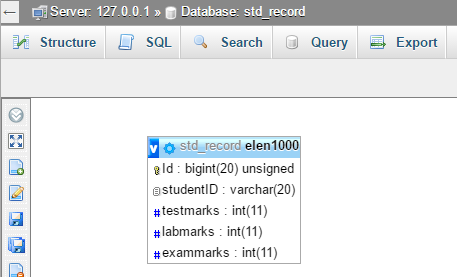
\includegraphics[width=8cm]{marks}
\caption{course table}
\end{figure}
\end{center}
  
\end{itemize}

\subsection{The application(Business model)}
PHP is  selected as a server scripting language. This language is chosen because of its simplicity, it is also a well documented programming language that is widely supported for web application development.

Interacting: the client tries logging in:

\begin{itemize}
\item Client enters credentials, these credentials get validated ‘onsubmit’.


\item If the credentials are correct: a PHP script is used to determine if the user is a  student or staff member.
\item If the user is a student then the student will only have certain privileges such as reading from the database only.
\item If the user is an administrator or a staff member then they may be allowed to have different privileges to edit the database: such as alter student results and add new students onto the database.
\end{itemize}

  


  % Back-End Documentation by Sanele Gcaba And Tshegofatso Misapitso


\section{Scrum Agile Method}

Scrum is a very quick and easy process which is widely used for managing and controlling software development projects in a rapidly changing environment. The aim of following the scrum methodology during a software development life cycle is to improve communication, maximise productivity, maximise cooperation amongst the team members and also controlling the chaos of conflicting interests. Scrum is a team based process and requires the co-operation of every member of the team \cite{SoftwareEngineering}. 


Each member of scrum needs to be a part in one of the three scrum roles namely the product owner, team member and a scrum master \cite{SoftwareEngineering}. 

\begin{itemize}
\item \textbf{Product Owner} \\
The product owner represents the stakeholders, customers and users. The product owner gives the goals of the project and the scrum team prioritises these as priorities of the project. The prioritized features will be selected and recorded in a product backlog. The Owner of the products needs to make sure that the project progresses and the project requirements are met. The project owner acts as a middle man between stakeholders and developers, he/she is also responsible of making plans and also announcing the release dates \cite{SoftwareEngineering}.    

\item \textbf{Team Members}
The team members are the developers of the software. The team must be organised and cross functional. The work to be done will be divided amongst the team members and also encourages the team to improve \cite{SoftwareEngineering}. 

    
\item \textbf{Scrum Master}

The scrum master solves all the problems and challenges that may be encountered during the course of the project \cite{SoftwareEngineering}. 
    
\end{itemize}  

In this project the Product owner is the lecturer, Etutu Otoo. He was responsible for issuing the projects requirements. The progress of the project was monitored by the product owner as submissions were made during the course of the project to monitor the success of the project.   

The Team members are the developers mentioned in the stakeholder diagram in section 1. In this project, the scrum master for the project was unanimously chosen to be the scrum master.  

\subsection{Sprint Planning } 

\subsubsection{Gantt chart}

The figures below show gantt charts for the project execution planning. 
  
\begin{center}
\begin{figure}[h]
\centering
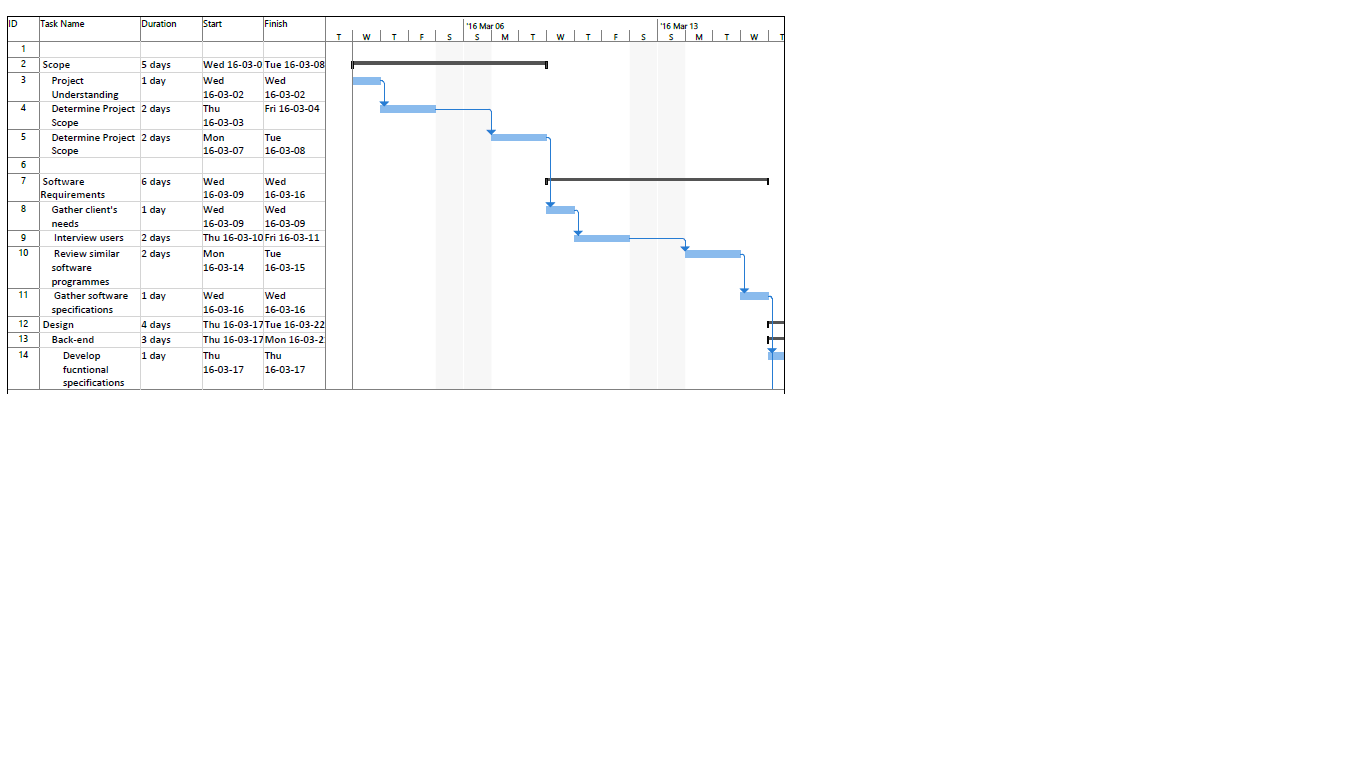
\includegraphics[trim = {0 10cm 14cm 0},clip, scale=0.58]{gantt1}
\caption{Gantt chart part 1}
\end{figure}
\end{center}


\begin{center}
\begin{figure}[h]
\centering
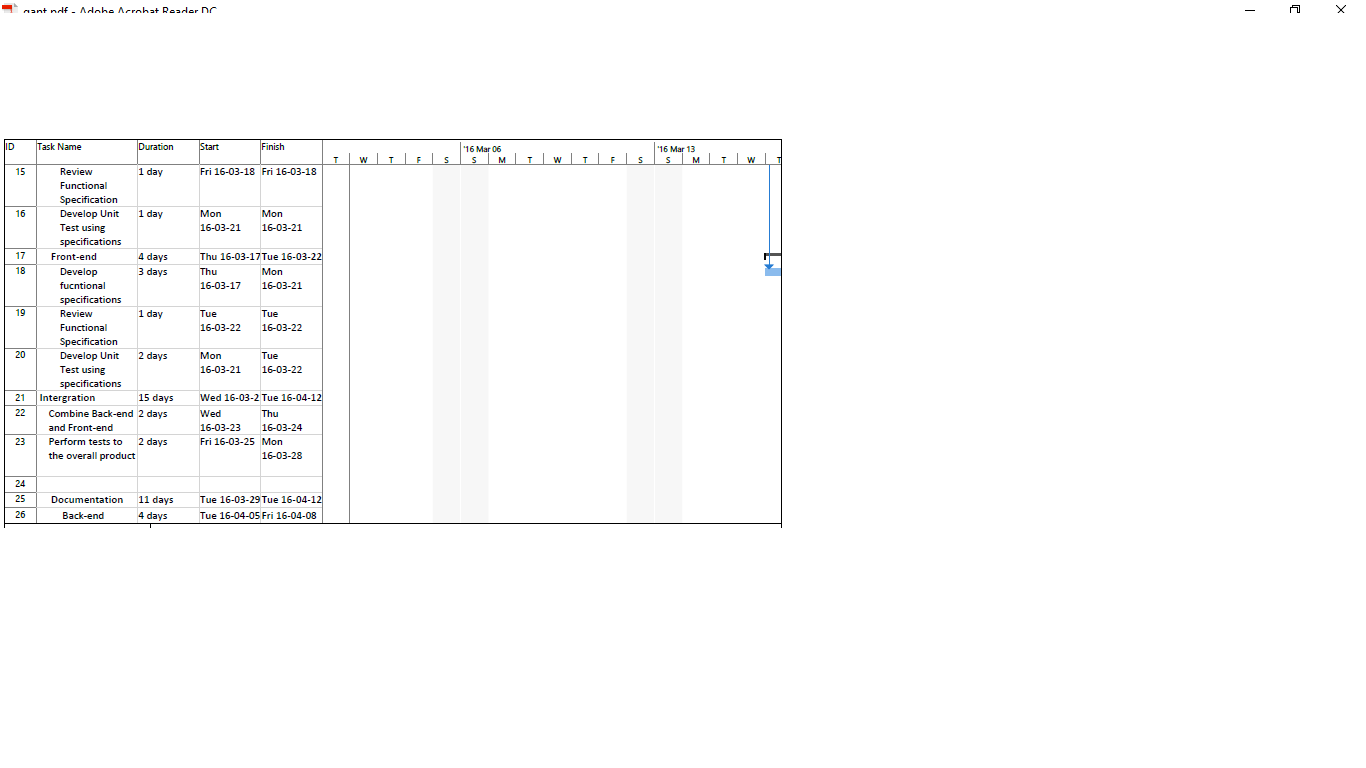
\includegraphics[trim = {0 6cm 14cm 2cm},clip, scale=0.58]{gantt2}
\caption{Gantt chart part 2}
\end{figure}
\end{center}


\begin{center}
\begin{figure}[h]
\centering
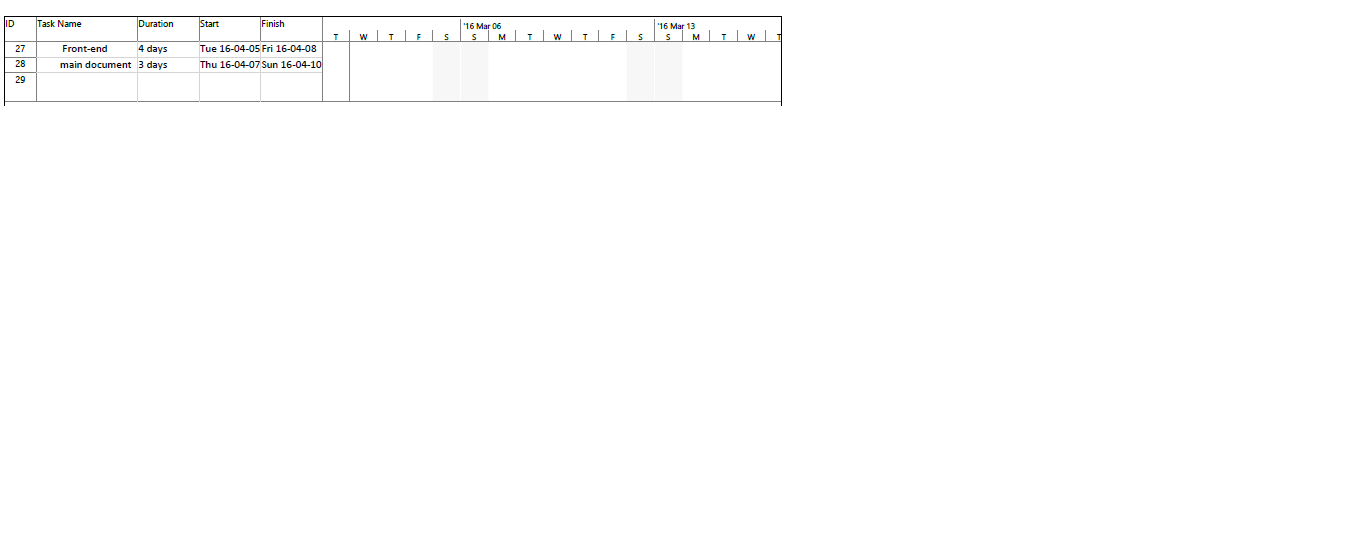
\includegraphics[trim = {0 11cm 14cm 0},clip, scale=0.58]{gantt3}
\caption{Gantt chart part 3}
\end{figure}
\end{center}

The gantt charts above were designed as a plan of action from the beginning of the project tasks until the end of the project, this gantt chart was developed directly from the requirement gathering process. Following this plan above and the owner's specifications, a product backlog list as shown in figure below was consequently developed. The backlog list shows priority of each individual task which was performed, following the list and daily scrum meetings that took 30 minutes, the task lists order of implementation were selected based on order of priority.      

\begin{center}
\begin{figure}[h]
\centering
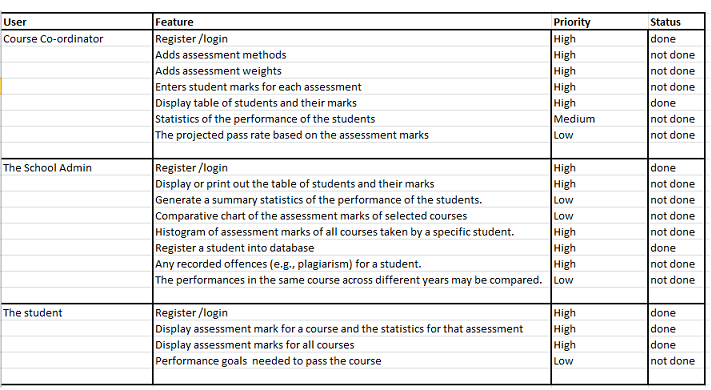
\includegraphics[trim = {0 0cm 0cm 0cm},clip, scale=1]{product_backlog}
\caption{Product backlog}
\end{figure}
\end{center}

\newpage
\subsubsection{Sprint Retrospective}~\\

Sprint retrospective serves to reflect on the current progress of the project to identify areas that need improvement and to reinforce good habits.

\textbf{Overall Sprint Retrospection}

	\begin{tabular}{ | p{5cm} | p{4cm} | }
		\hline
		\textbf{Well done} & \textbf{future improvement}\\ \hline
		Co-ordination 	& Scrum meetings were effective but took longer than planned quite often\\ \hline	
		Effective communication& Under-estimation of tasks \\ \hline
		Punctuality & Uneven work distribution			
		\\ \hline
	\end{tabular}
	
The figure below shows that the estimated time was not followed precisely as highlighted in the improvement section above.	
	
\begin{center}
\begin{figure}[h]
\centering
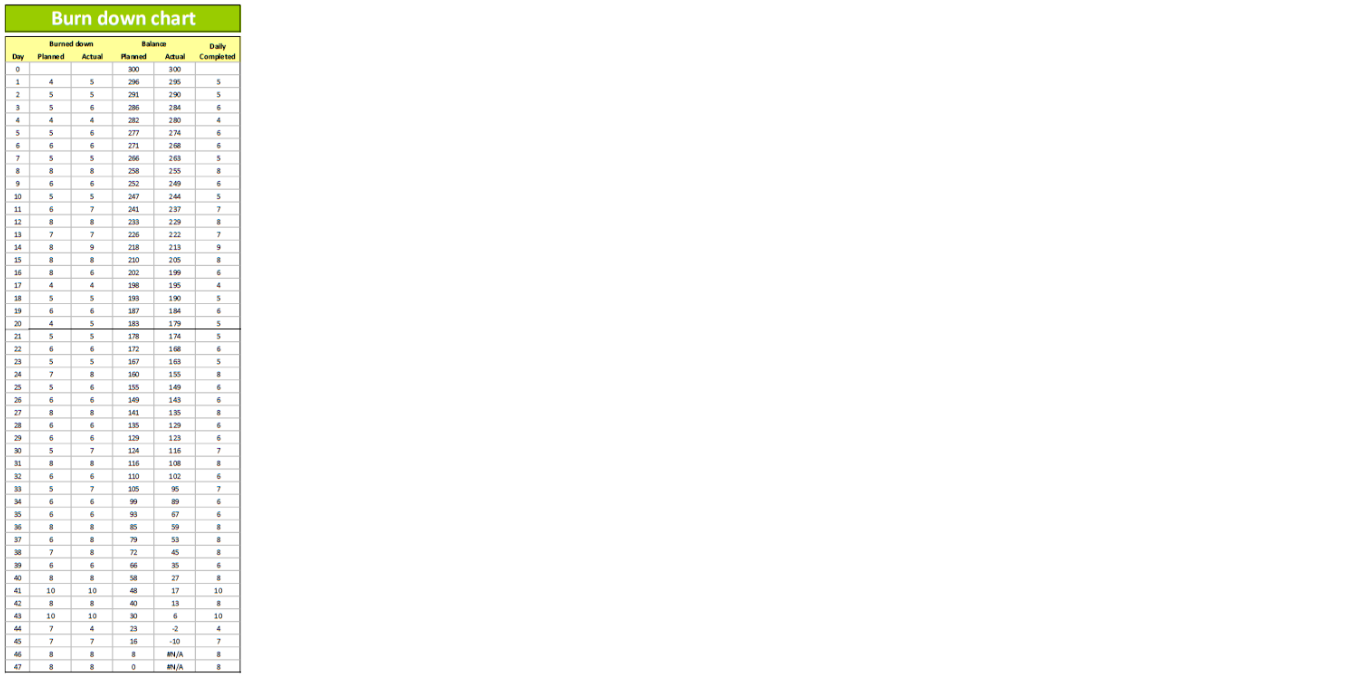
\includegraphics[trim = {0 0cm  28cm 0cm},clip, scale=0.7]{burndown1}
\caption{Burn down chart data}
\end{figure}
\end{center}

\begin{center}
\begin{figure}[h]
\centering
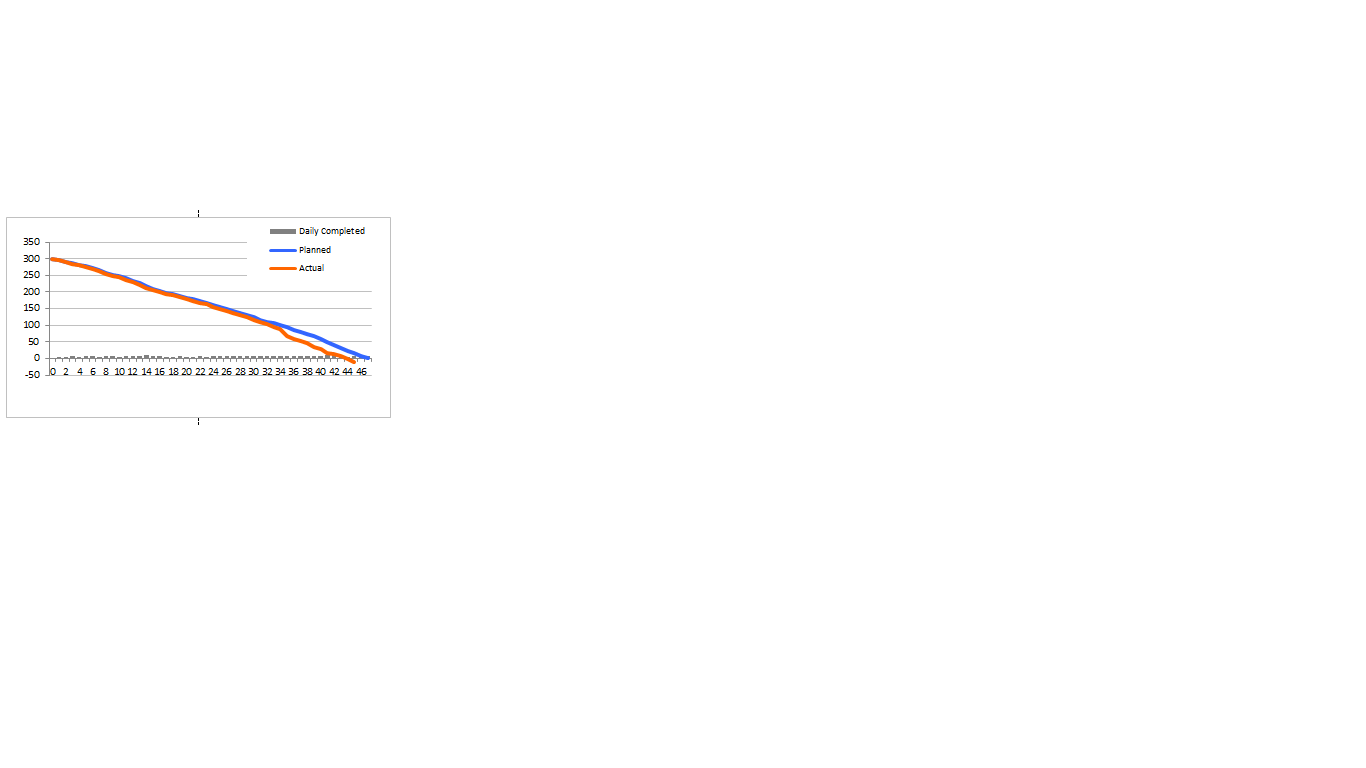
\includegraphics[trim = {0 8.5cm 25cm 4.5cm},clip, scale=1]{burndown}
\caption{Burn down chart}
\end{figure}
\end{center}

\clearpage
\section{Description of some relevant(demonstrable) module}

The login page is shown in Figure 27. The users are able to select the domain on the drop-down as shown in Figure 27. If the login details valid the user will either be redirected to a student page, course coordinator page or an administrator page depending on the domain specified. 

\subsection{Login page}
\begin{center}
\begin{figure}[h]
\centering

\includegraphics[trim = {0 0cm 0cm 0cm},clip, scale=0.5]{loginPage}
\caption{Login page}
\end{figure}
\end{center}

\newpage 

The student page is shown in Figure 28

\subsection{Student page}
\begin{center}
\begin{figure}[h]
\centering
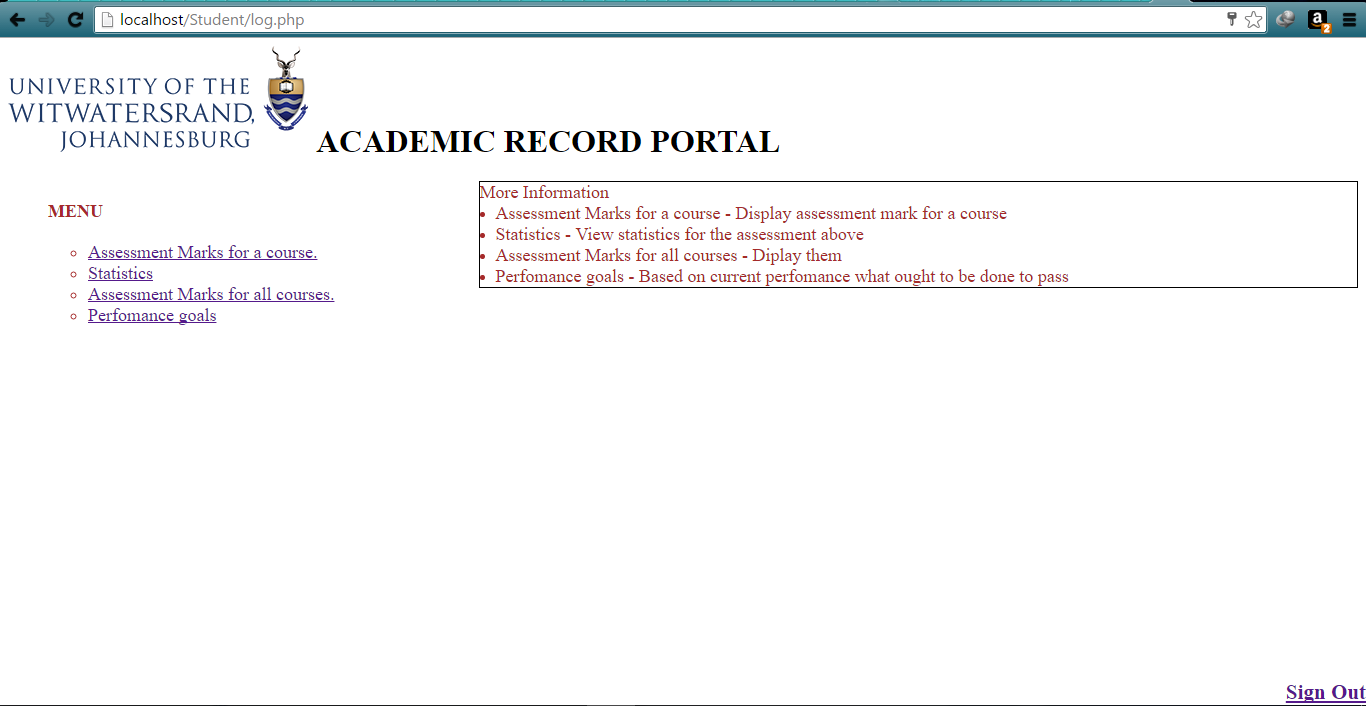
\includegraphics[trim = {0 0cm 0cm 0cm},clip, scale=0.5]{studentPage}
\caption{Student page}
\end{figure}
\end{center}



When the student clicks on display marks for all courses option he/she will be redirected to a page where final marks for each courses will be shown as can be seen in Figure 29. 

\newpage
\begin{center}
\begin{figure}[h]
\centering
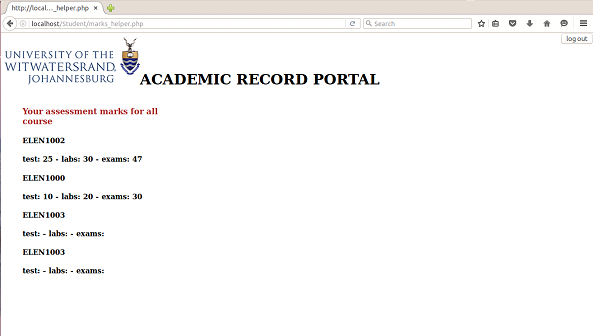
\includegraphics[trim = {0 0cm 0cm 0cm},clip, scale=1]{StudentMarks}
\caption{display marks for all courses page}
\end{figure}
\end{center}

\newpage
\subsection{Course coordinator home page}

The course coordinator home page is shown in figure 30.

\begin{center}
\begin{figure}[h]
\centering
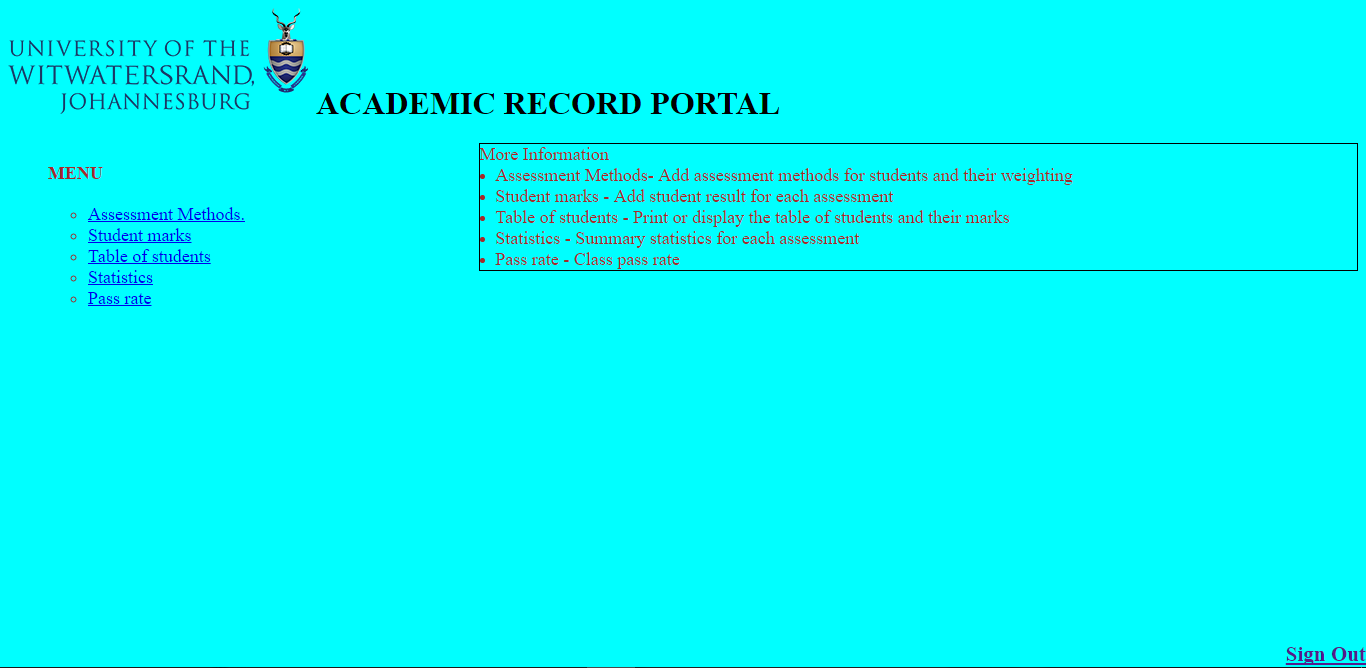
\includegraphics[trim = {0 0cm 0cm 0cm},clip, scale=0.5]{CourseCoordinatorPage}
\caption{Course coordinator page}
\end{figure}
\end{center}

When the click assessment methods, he is redirected to a page where he can add a course as shown in Figure 31.


\begin{center}
\begin{figure}[h]
\centering
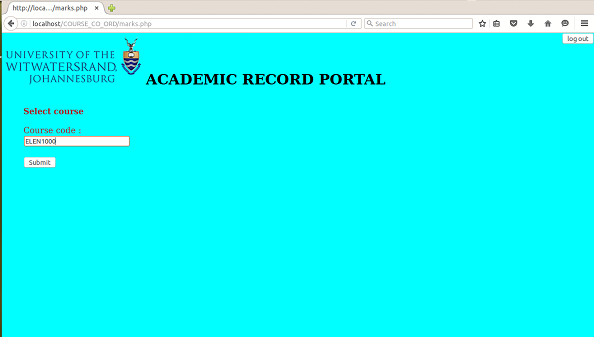
\includegraphics[trim = {0 0cm 0cm 0cm},clip, scale=1]{RegisteringAcourse}
\caption{Registering a course}
\end{figure}
\end{center}

\newpage

\section{Administrator page}

The administrator page is shown i Figure 32. 


\begin{center}
\begin{figure}[h]
\centering
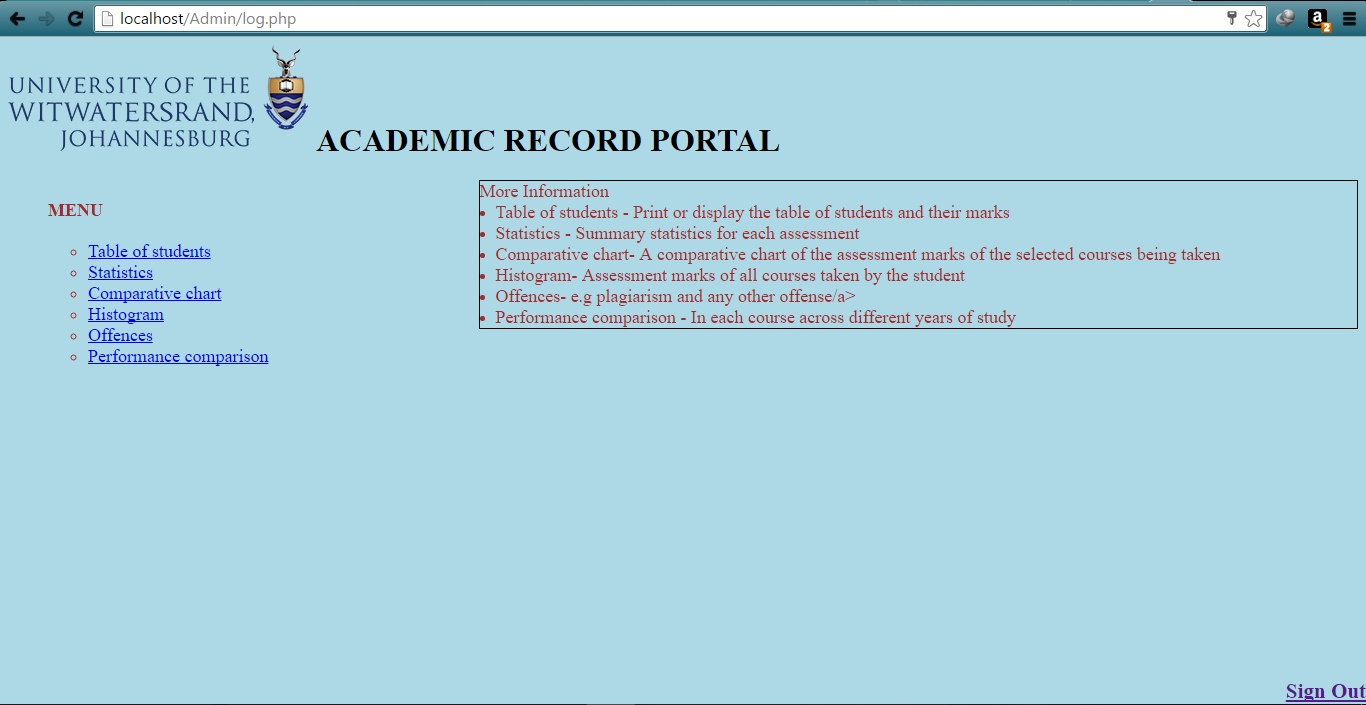
\includegraphics[trim = {0 0cm 0cm 0cm},clip, scale=0.5]{AdminPage}
\caption{Administrator page}
\end{figure}
\end{center}

The administrator is able to register a student when he/she clicks the table of students option as shown in Figure 33. 


\begin{center}
\begin{figure}[h]
\centering
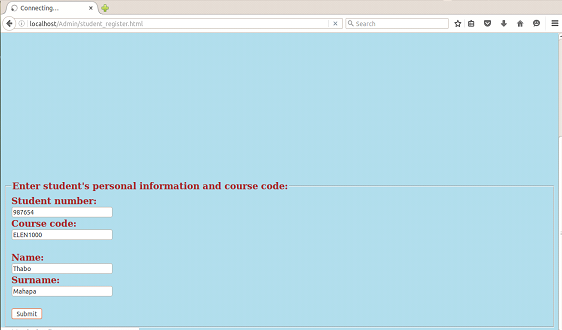
\includegraphics[trim = {0 0cm 0cm 0cm},clip, scale=1]{RegisteringStudents}
\caption{Students registering page}
\end{figure}
\end{center}


\newpage
\clearpage

\section{Conclusion}

The student record/marks system is presented in this document. With the aim of developing and implementing the system, project requirements are established and the design of the system is separated into the front-end and back-end subsystems. The scrum agile method is chosen as the (SDLC) methodology to quickly deliver a working prototype. As shown in the product backlog not all features were successfully implemented due to time constrains and their complexity.   

\newpage
%\nocite{*}
\bibliographystyle{witseie}
\bibliography{sample}

%{\tiny \vfill \hfill \today \hspace{5mm} witseie-paper-2003.\TeX}

\end{document}

" vim: ts=4
" vim: tw=78
" vim: autoindent
" vim: shiftwidth=4
file:///C:/Users/masana khosa/Desktop/SoftWareEngReport/Stakeholders.PNG